% !TEX encoding = UTF-8
% !TEX TS-program = pdflatex
% !TEX root = ../tesi.tex
%**************************************************************
\chapter{Discussione e comparazione dei risultati}
\label{cap:precls}
%**************************************************************
\intro{In questo capitolo si discuteranno i risultati ottenuti dai modelli di Bradley-Terry e dalle tecniche di Machine Learning. Si concluderà con una comparazione tra i risultati delle tecniche di Data Mining e di Machine Learning.
}
%**************************************************************
\section{Discussione risultati dei modelli Bradley-Terry}
Come illustrato nel Capitolo \ref{cap:risultatiDM} sono state applicate quattro versioni del modello Bradley-Terry. Con la prima versione, ovvero il modello Bradley-Terry standard con effetti dell'ordine (\hyperref[for:3.9]{4.9}) \autocite{bradley1952rank} è stato possibile stimare l'abilità di ogni singola squadra e l'effetto di giocare in casa, costruendo così, una base da cui partire per ottenere risultati più esplicativi. Infatti, con l'introduzione di 26 covariate nelle comparazioni ovvero, con il modello (\ref{for:5.1}), è stato possibile approfondire in che modo le variabili esplicative sono associate all'esito di una partita. Successivamente per abbassare la complessità del modello e per analizzare che stima viene associata ad ogni covariata per ogni squadra, nel modello (\ref{for:4.9}) è stato introdotto e applicato il metodo di regolarizzazione LASSO. Per approfondire gli effetti delle singole variabili esplicative a seconda della squadra in esame è stato applicato il modello (\ref{for:5.2}) in cui viene tolto l'effetto dell'intercetta. Si sottolinea inoltre che, come spiegato nel Capitolo \ref{cap:extraDM}, per utilizzare le variabili esplicative gol fatti \texttt{GF} e gol subiti \texttt{GA} è stato riapplicato il modello (\hyperref[for:3.9]{4.9}) ma con una variabile risposta \emph{Y} con cinque categorie invece che tre. Tale modello a livello di stime ha prodotto risultati simili al modello (\hyperref[for:3.9]{4.9}) con \emph{Y = 3}, con solo piccole differenze, permettendo così di raffinare l'analisi.\\
Dai risultati ottenuti è possibile concludere quanto segue. Nel campionato italiano, ai fini della vittoria o, in generale, dell'ottenimento di buoni risultati, è rilevante per una squadra adottare un comportamento tattico, in particolare la costruzione dal basso, e giocare prevalentemente nella propria metà campo. 
È importante che la squadra adotti un comportamento meno propenso a controllare il pallone per lungo tempo perché sia il possesso della palla \texttt{Poss} sia la distanza percorsa con la palla \texttt{TotDist} non risultano essere vantaggiosi. La squadra deve essere più propensa a giocare la palla nella propria area di difesa per evitare contropiedi perché le stime del numero di tocchi in area di rigore \texttt{ToDefPen}, il numero di tocchi nella trequarti difensiva \texttt{ToDef3rd} e il numero di tocchi a centrocampo \texttt{ToMid3rd} sono associati ad un aumento della probabilità di vittoria. Perciò, avere una buona difesa è fondamentale. La fase offensiva non deve essere troppo lunga in termini di possesso della palla. Infatti, il numero di tocchi fatti nella trequarti offensiva \texttt{ToAtt3rd} porta ad avere una diminuzione delle probabilità di vittoria. Se però, si fanno i giusti passaggi per entrare nell'area di rigore avversaria mantenendo sempre un possesso palla breve si aumentano le probabilità di vittoria. Considerando i casi di Inter e Atalanta, %vedi grafico
la prima si dimostra essere una dalle squadre che più tira in generale (\texttt{Sh}) e in porta (\texttt{SoT}). Alti valori sono presenti anche per l'Atalanta. Entrambe però mantengono troppo il controllo del pallone nell'area avversaria. Infatti, per entrambe le squadre si riscontrano notevoli diminuzioni della probabilità di vittoria a causa della stima del parametro di \texttt{ToAtt3rd}. Peggio ancora per l'Atalanta, che ha un gioco particolarmente offensivo (vedi \textit{\cite{ataGioco}}), che le fa ottenere una diminuzione della probabilità della vittoria dalla stima del parametro \texttt{ToAttPen}, diversamente dalle altre squadre dove la stima è leggermente positiva. Questo perché il prolungato controllo del pallone la porta a esporsi e a subire il contropiede. Si è parlato spesso di contropiedi nella nostra analisi. Quello che emerge sempre in tema di fase offensiva è che il numero di tiri è relativamente basso, fatto dimostrato dal notevole aumento della probabilità di vittoria portato della stima del rapporto gol/tiri \texttt{G/Sh}. Di conseguenza le squadre attaccano poco e, quando lo fanno, cercano di massimizzare la loro fase offensiva. Infatti, le partite nel campionato italiano, spesso finiscono con un massimo di due o tre gol segnati. Pertanto, l'efficacia di un azione offensiva che porta al gol e la carenza di azioni offensive portano \texttt{Sh}, \texttt{SoT}, ma soprattutto \texttt{G/Sh}, ad assumere un elevato contributo nel determinare la vittoria.\\
Concludendo la trattazione sulla fase offensiva, si illustra quale sia il miglior modo di attaccare che emerge dai modelli. Si sa che il contropiede è efficace, ma allo stesso tempo difficile da attuare per via del comportamento delle squadre a non sbilanciarsi. Una valida alternativa che emerge è il lancio lungo che parte dall'area compressa tra l'area di rigore della squadra fino a centrocampo ed arriva nell'area avversaria. Infatti, la stima del parametro del numero di passaggi lunghi tentati \texttt{LPAtt} è associata ad una crescita della probabilità di vittoria. L'utilizzo di passaggi filtrati \texttt{MPCmp\%} non è una buona tattica dato che esso risulta associato a una diminuzione della probabilità di vittoria per tutte le squadre. Analogamente, i cross \texttt{Crs} sono associati a una diminuzione della probabilità di vittoria per tutte le squadre. Nello specifico, vengono leggermente più penalizzate Roma, Milan, Napoli mentre vengono particolarmente penalizzate Inter e l'Atalanta, squadra che con il suo gioco sfrutta molto le fasce (vedi \textit{\cite{ataGioco}}). Il fuorigioco risulta essere associato a una diminuzione della probabilità di vittoria per le squadre con l'abilità maggiore in particolare Milan, Napoli, Inter e Juventus. In conclusione, è importante sottolineare che un atteggiamento troppo speculativo o difensivo da parte della squadra non porta alla vittoria. Questo è il caso del Venezia, classificatosi come ultimo, e che ha ottenuto benefici dalle covariate \texttt{ToDefPen} e \texttt{ToDef3rd}, ma non dalle variabili esplicative offensive. Perciò, dall'analisi emerge che per ottenere la vittoria una squadra debba mantenere un comportamento tattico e giocare prevalentemente nella propria metà campo.\\
Infine, ogni modello ha prodotto delle predizioni dei risultati di alcune partite. Si sono confrontate le prestazioni dei cinque modelli durante la fase di test insieme alle predizioni fatte dai \emph{bookmakers}. Quello che si evince è che tutti i modelli Bradley-Terry hanno prestazioni migliori delle predizioni dei \emph{bookmakers}, segno che le informazioni vengo utilizzate in modo opportuno. Purtroppo, non sono soddisfacenti in termini di predizioni. Infatti, si ottengono delle discrete prestazioni dal punto di vista dell'accuratezza, precisione, sensibilità e della specificità. Il modello Bradley-Terry che ha ottenuto le migliori prestazioni in fase di predizione è stato (\ref{for:4.9}), ma con la variabile risposta \emph{Y} a cinque categorie. Il modello (\ref{for:4.9}) è il modello con le covariate specifiche del soggetto e dell'oggetto con effetto specifico dell'oggetto. Infatti, con questa modifica si va a migliorare le prestazioni del modello (\ref{for:4.9}) che già risultava essere il più accurato con \emph{Y = 3}.
\section{Discussione risultati dei modelli di Machine Learning}
Gli algoritmi di apprendimento automatico scelti sono stati utilizzati per predire l'esito di un insieme di partite, ovvero classificare le partite con una delle seguenti classi: vittoria della squadra in casa, pareggio o vittoria della squadra ospite.\\
Gli algoritmi utilizzati sono il K-Nearest-Neighbors (K-NN), la Support Vector Machine (SVM), il Decision Tree, la Random Forest e l'AdaBoost. L'algoritmo K-NN è stato scelto perché è semplice da implementare e rapido nell'esecuzione. L'algoritmo SVM è spesso impiegato grazie all'utilizzo del \emph{kernel trick} che permette all'algoritmo di adattarsi bene in vari contesti. Per questa ragione si è deciso di applicare la SVM. L'algoritmo Decision Tree, oltre a essere semplice da implementare e molto usato, è stato scelto anche per individuare quali sono le \emph{features} più decisive per la predizione. Infine, sono stati scelti gli algoritmi Random Forest e AdaBoost perché entrambi sono due tecniche di apprendimento \emph{ensemble} ma con filosofie differenti. Inoltre, il Random Forest permette di individuare quali \emph{features} danno maggior guadagno di informazioni.\\
Grazie alla metrica AUC è possibile confrontare le performance degli algoritmi utilizzati. Nella Figura \ref{fig:auc} vengono riportate le AUC che sono state misurate durante la fase di predizione di ogni algoritmo utilizzato.
\begin{figure}[h]
	\begin{center}
		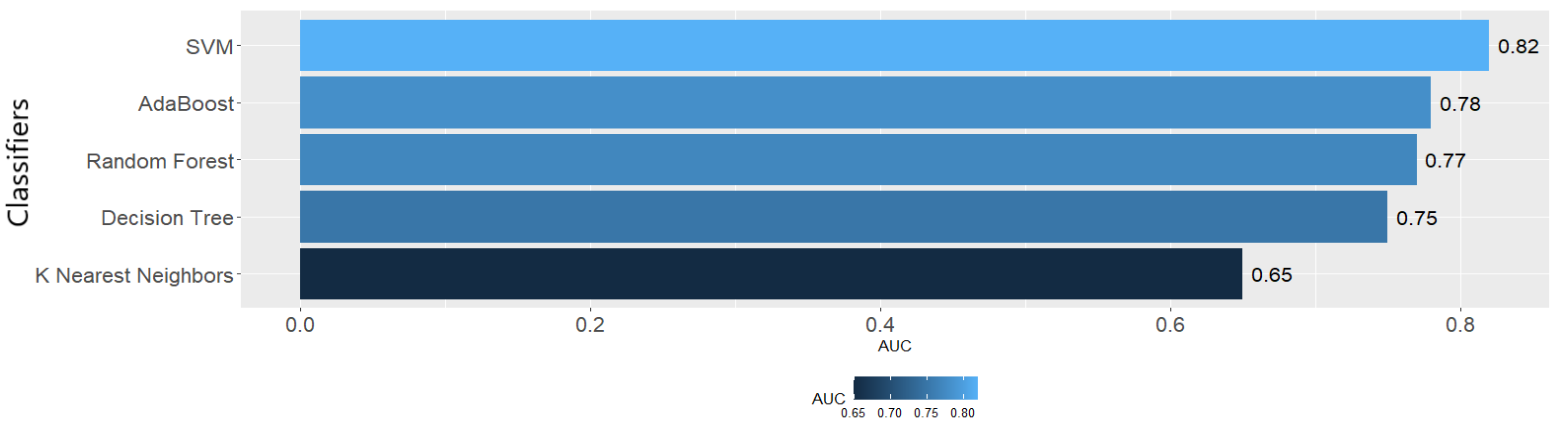
\includegraphics[scale=0.30]{auc.png}
		\caption{Grafico a barre in cui viene riportata la Area Under the Curve (AUC) registrata durante la fase di predizione degli algoritmi K-Nearest-Neighbors (K-NN), Support Vector Machine (SVM), Decision Tree, Random Forest e AdaBoost.  
		} 
		\label{fig:auc}
	\end{center}
\end{figure}
Dalle misurazioni ottenute si evince che l'AUC più alta è stata registrata nell'algoritmo SVM con un valore pari a 0.82. Infatti, la SVM ha una buona accuratezza perché è l'algoritmo che riesce a identificare con maggior precisione la classe pareggio, la quale è risultata molto ostica da identificare per gli algoritmi trattati. Con una AUC leggermente inferiore, l'algoritmo AdaBoost si classifica come secondo con un valore pari a 0.78. Analogamente alla SVM, l'AdaBoost si distingue dagli algoritmi con prestazioni inferiori grazie alle discrete prestazioni nell'identificazione della classe pareggio. L'algoritmo con la terza AUC più alta è stato il Random Forest con una AUC pari a 0.77 e con prestazioni simili all'algoritmo AdaBoost.
In quarta posizione si piazza l'algoritmo Decision Tree con una AUC pari a 0.75. Nonostante le buone prestazioni registrate nell'identificazione delle classi vittoria della squadra in casa e vittoria della squadra ospite, l'algoritmo Decision Tree paga una minor AUC a causa delle brutte prestazioni registrate nell'identificazione della classe pareggio. Infine, l'algoritmo con la più bassa AUC misurata è il K-NN con una AUC pari a 0.65. Infatti, l'algoritmo K-NN ha registrato delle pessime prestazioni nell'identificare le istanze di classe pareggio e delle discrete prestazioni nell'identificare le istanze delle altre due classi.\\
In conclusione, il problema presentato risulta essere troppo complesso per l'algoritmo K-NN: la strategia di classificare una nuova istanza con la classe di maggioranza dei k-vicini, seppur semplice, non è risultata efficace. Viceversa, la SVM, grazie all'utilizzo della funzione kernel, riesce a gestire la complessità dei dati ottenendo delle buone prestazioni in fase di predizione.
\section{Confronto}
Come riportato riportato dalla Tabella \ref{tab:acc} in cui vengono riportate le accuratezze registrate nel \emph{validation set} durante la fase di \emph{training} e nel \emph{test set} durante la fase di predizione, le prestazioni migliori in fase di predizioni si ottengono con i metodi di \emph{Machine Learning}. 
\begin{table}[!ht]
	\begin{longtable}{|C{0.18\textwidth}|C{0.17\textwidth}|C{0.17\textwidth}|}
		\hline	
		\rowcolor{SchoolColor2}
		\textbf{Procedura} & \textbf{Accuratezza Training} & \textbf{Accuratezza Test}\\
		\hline			
		BTM & 0.67 & 0.65 \\
		\hline	
		BTMG & 0.65 & 0.61\\
		\hline	
		BTM3O + LASSO & 0.68 & 0.66 \\
		\hline	
		BTM5O + LASSO & 0.69 & 0.68 \\
		\hline	
		BTMNI3O + LASSO & 0.65 & 0.63 \\
		\hline	
		K-NN & 0.58 & 0.58\\
		\hline	
		SVM & 0.79 & 0.78 \\
		\hline	
		Decision Tree & 0.68 & 0.71 \\
		\hline	
		Random Forest & 0.75 & 0.72\\
		\hline	
		AdaBoost & 0.78 & 0.72 \\
		\hline
	\end{longtable}	
	\vspace*{5mm}
	
	\caption{La tabella riporta l'accuratezza registrata nel \emph{validation set} durante la fase di training e nel \emph{test set} durante la fase di predizione. BTM = modello Bradley-Terry standard con effetto d'ordine. BTMG = modello BT con covariate specifiche del soggetto e dell'oggetto con effetto globale. BTM3O + LASSO = modello BT con variabile risposta \emph{Y} a tre categorie, covariate specifiche del soggetto dell'oggetto con effetto specifico dell'oggetto, con LASSO. Con BTMNI3O + LASSO = modello BT senza intercette, con variabile risposta \emph{Y} a tre categorie, covariate specifiche del soggetto dell'oggetto con effetto specifico dell'oggetto, con LASSO. K-NN = K-Nearest-Neighbors. SVM = Support Vector Machine.} \label{tab:acc}
\end{table}
I modelli di \emph{Data Mining} sono utili per interpretare le relazioni tra le variabili, meno in termini di predizioni. Ciononostante, grazie all'interpretabilità dei modelli è possibile individuare quali variabili siano associate all'esito della partita e in che misura. Viceversa, i modelli di \emph{Machine Learning} in genere, si focalizzano su caratteristiche troppo complesse e difficili da interpretare. Grazie agli algoritmi Decision Tree e Random Forest è comunque possibile fare un confronto con i modelli Bradley-Terry riguardo a quali variabili siano associate all'esito della partita.
Notiamo che le variabili legate ai tiri sono le più importanti per entrambi i modelli. Nei due modelli di \emph{Machine Learning} viene data molta importanza sia ai passaggi lunghi tentati, come per i modelli BT, sia alla percentuale di passaggi lunghi completati in contrasto con i modelli BT. 
Sia i modelli BT e sia i modelli Decision Tree e Random Forest, la \emph{feature} della percentuale dei passaggi medi completati ricopre un ruolo importante nell'esito della partita. Tuttavia, dai modelli BT sappiamo che essa è associata negativamente sulla probabilità di vittoria.
Nonostante tante similitudini tra i risultati delle due tipologie di metodi, ci sono alcune differenze. Si hanno differenze di interpretazioni sull'importanza del numero di parate. Per il modello Bradley-Terry la variabile si associa fortemente all'esito della partita, mentre per i due modelli di \emph{Machine Learning} no. Viceversa, la percentuale di passaggi completati è molto importante per i  modelli di \emph{Machine Learning}, mentre non lo è per i modelli BT. Anche per la distanza percorsa con la palla viene assegnato un rilevante guadagno di informazione, solo nei modelli di \emph{Machine Learning}. Per entrambi i metodi viene ribadita la poca importanza riguardo al possesso della palla e delle variabili riguardanti il numero di contrasti vinti e il numero di intercetti. Anche i numeri di falli subiti e fatti non hanno una grande importanza per entrambi i metodi. Inoltre, per entrambi i metodi il numero di falli fatti è leggermente più rilevante rispetto al numero di falli subiti.\\
Dal punto di vista dei tempi d'esecuzione si segnala una maggior velocità di esecuzione dei modelli Bradley-Terry rispetto ai modelli di \emph{Machine Learning}. In particolare, l'algoritmo Random Forest impiega il maggior tempo d'esecuzione fra tutti gli algoritmi.


